\documentclass[11pt]{beamer}
\setbeamertemplate{navigation symbols}{}
 \setbeamercovered{transparent}
\usepackage{listings}
%\usetheme{Copenhagen}
\usetheme{Singapore}
%\usetheme{Madrid}
%\usetheme{Hannover}
%\usetheme{boxes}
%\usetheme{Boadilla}
\usefonttheme[onlymath]{serif}
\usecolortheme{beaver}
\usepackage{textpos}
\usepackage{fancyvrb}
\usepackage{xcolor}
\usepackage{multicol}
\usepackage{lipsum}
\parskip 1ex

\newcommand\FontAcolumn{\fontsize{6}{7.2}\selectfont}
\newcommand\FontBcolumn{\fontsize{8}{7.2}\selectfont}
\newcommand\FontCcolumn{\fontsize{10}{7.2}\selectfont}
\newcommand\FontDcolumn{\fontsize{11}{7.2}\selectfont}

\definecolor{gray97}{gray}{.97}
\definecolor{gray75}{gray}{.75}
\definecolor{gray75}{gray}{.45}

\lstdefinestyle{Fortran}{language=[90]Fortran}

\newcommand\FortranStyle
{
\lstset{
frame=Ltb,
framerule=0pt,
columns=fullflexible,
aboveskip=0.5cm,
framextopmargin=3pt,
framexbottommargin=3pt,
framexleftmargin=0.4cm,
framesep=0pt,
rulesep=.4pt,
backgroundcolor=\color{gray97},
rulesepcolor=\color{black},
stringstyle=\ttfamily,
showstringspaces=false,
basicstyle=\ttfamily,
commentstyle=\color{green},
keywordstyle=\color{red},
numbers=left,
numbersep=15pt,
numberstyle=\tiny,
numberfirstline=false,
breaklines=true,
 tabsize=2,
 extendedchars=true,
keepspaces,
}
}

\newcommand\FortranStyleA
{
\lstset{
frame=Ltb,
framerule=0pt,
columns=fullflexible,
aboveskip=0.5cm,
framextopmargin=3pt,
framexbottommargin=3pt,
framexleftmargin=0.4cm,
framesep=0pt,
rulesep=.4pt,
backgroundcolor=\color{gray97},
rulesepcolor=\color{black},
stringstyle=\ttfamily,
showstringspaces=false,
basicstyle=\ttfamily,
commentstyle=\color{green},
keywordstyle=\color{red},
numbersep=15pt,
numberstyle=\tiny,
numberfirstline=false,
breaklines=true,
 tabsize=2,
 extendedchars=true,
keepspaces,
}
}

\newcommand\tab[1][1cm]{\hspace*{#1}}
\newcommand{\light}[1]{\textcolor{lightgray}{#1}}
    
\def\signed #1{{\leavevmode\unskip\nobreak\hfil\penalty50\hskip2em
  \hbox{}\nobreak\hfil(#1)%
  \parfillskip=0pt \finalhyphendemerits=0 \endgraf}}

\newsavebox\mybox
\newenvironment{aquote}[1]
  {\savebox\mybox{#1}\begin{quote}}
  {\signed{\usebox\mybox}\end{quote}}
  
% items enclosed in square brackets are optional; explanation below
\title{$1^{st}$ NASA LRC Fortran Tutorial}
\subtitle{Introduction and Setup}
\author{Carlos Cruz\\
Jules Kouatchou\\
Bruce Van Aartsen}
\institute{
  NASA GSFC Code 606 (ASTG)\\
  Greenbelt, Maryland 20771\\[1ex]}
\date{October 24-25, 2018}

\begin{document}

% --- Title page ---
\begin{frame}[plain]
  \titlepage
\end{frame}

\logo{%
  
\includegraphics[width=1cm,height=1cm,keepaspectratio]{../../shared/nasa-ball.png}%
  \hspace{\dimexpr\paperwidth-2cm-5pt}%
  
\includegraphics[width=1cm,height=1cm,keepaspectratio]{../../shared/ssai-logo.png}%
}

% --- Slide

\begin{frame}{Who we are?}

\begin{itemize}
    \item Carlos Cruz (Computational Scientist)
    \item Jules Kouatchou (Computational Scientist)
    \item Bruce Van Aartsen (Senior Software Engineer)
\end{itemize}
We are members of the Advanced Software Technology Group (ASTG) Code 606, NASA GSFC.

\end{frame}

% --- Slide

\begin{frame}{Agenda}

\begin{columns}[onlytextwidth,t]
    \begin{column}{0.48\textwidth}
        \textbf{Day 1}

    \begin{itemize}
        \item \textcolor{red}{Introduction to Fortran}
        \item \textcolor{blue}{Variables and data types
        \item Conditionals and loops
        \item Array concepts
        \item Subroutines and functions
        \item Modules and interfaces
        \item File IO}
    \end{itemize}
  \end{column}
  \begin{column}{0.48\textwidth}
    \textbf{Day 2}

    \begin{itemize}
        \item \textcolor{blue}{Derived types and pointers}
        \item \textcolor{green}{Introduction to OOP
        \item IO Enhancements
        \item Inheritance
        \item Polymorphism
        \item Miscellaneous items
        \item Interoperability with C}
    \end{itemize}
  \end{column}
\end{columns}

\begin{center}
\textcolor{blue}{Introduction to Fortran 90-95}\\
\textcolor{green}{Introduction to Fortran 2003}
\end{center}

\end{frame}

% --- Slide

\begin{frame}{Get Lecture Materials from Github}
\footnotesize{Open a terminal (Linux/Mac) or command prompt (Windows) and use Git:\\}
\footnotesize{\quad git clone \url{https://github.com/cacruz/LRC_Fall18_Fortran.git}}\\
\vspace{5mm}
If Git is not available or Git is not working then, in your browser open \url{https://github.com/cacruz/LRC_Fall18_Fortran.git}, and download the zip file.
\begin{figure}[t]
\centering
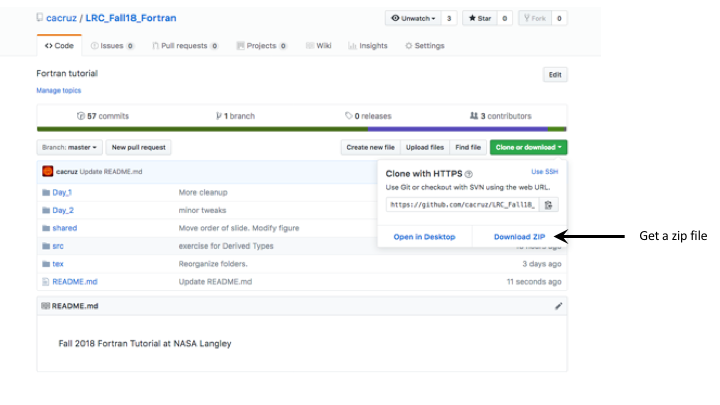
\includegraphics[scale=.25]{../../shared/github_zip}
\end{figure}

\end{frame}

% --- Slide

\begin{frame}[fragile]
\frametitle{Log in to Amazon EC2}

\footnotesize{Open a terminal (Linux/Mac) or command prompt (Windows) and go into the LRC\_Fall18\_Fortran directory/amazon (what you just downloaded):}

\tiny{
\begin{Verbatim} 
cd LRC_Fall18_Fortran/amazon
ssh -i "fortranlrc.pem" <student>@ec2-18-217-60-67.us-east-2.compute.amazonaws.com

substitute <student> for your assigned userid
\end{Verbatim}
}
\footnotesize{If your ssh command is successful then get the Fortran code in your Amazon account:}
\scriptsize{
\begin{Verbatim} 
$ git clone https://github.com/cacruz/LRC_Fall18_Fortran.git
$ cd LRC_Fall18_Fortran/src
$ ls
01_Introduction
02_Data_types
03_Control_constructs
04_Array_concepts
etc...
\end{Verbatim}
}
\begin{center}
\textbf{If possible, leave terminal -with ssh connection- open for the rest of the day.}
\end{center}
\end{frame}


\end{document}
